\subsubsection{Installieren und Konfigurieren der Software auf den WS}
    \textbf{Planung}
    \begin{itemize}
        \item Zwei Win 8 Rechner starten
        \item Rechner per P2P verbinden
        \item Auf einer Maschine XAMPP installieren mit Auswahl nur Apache, auf der zweiten Maschine Wireshark installieren
        \item Auf beiden PC's Firewall deaktivieren
        \item DHCP auf statische IP’s umstellen: 10.0.0.2 \& 10.0.0.3
        \item Im xampp-Verzeichnis unter htdocs  die Seite hallo.htm einfügen
        \item Im browser die Seite über “localhost/hallo.htm” und “<IP>{\textbackslash}hallo.htm” aufrufen
    \end{itemize}
    \vspace{0cm}
    \underline{\textbf{DoD Schichtmodel}}\\
    \textbf{Network Access Schicht}\\
    (Die Schicht, auf der die Geräte physisch verbunden sind)
    \begin{itemize}
        \item Bei uns über internen virtuellen Switch gelöst
        \item MAC Adresse wird ausgelesen
    \end{itemize}
    \vspace{0cm}
    \textbf{Internet Schicht}
    (Die Schicht, die Netzwerkweite Verbindungen unabhängig von Übertragungsmedium ermöglicht)
    \begin{itemize}
        \item IP Adresse wird ausgelesen
    \end{itemize}
    \vspace{0cm}
    \textbf{Host to Host Schicht}
    (Die Schicht, die den Tranbsport von Daten und eine Peer to Peer Verbindung ermöglicht)
    \begin{itemize}
        \item Haben wir über Arbeitsgruppe ermöglicht
    \end{itemize}
    \vspace{0cm}
    \textbf{Process}
    (Die Schicht, die die tatsächlichen Nutzdaten entsprechend den jeweiligem Protokoll ablegt)
    \begin{itemize}
        \item Ist bei uns via HTTP
    \end{itemize}
    
    \begin{figure}[H]
        \centering
        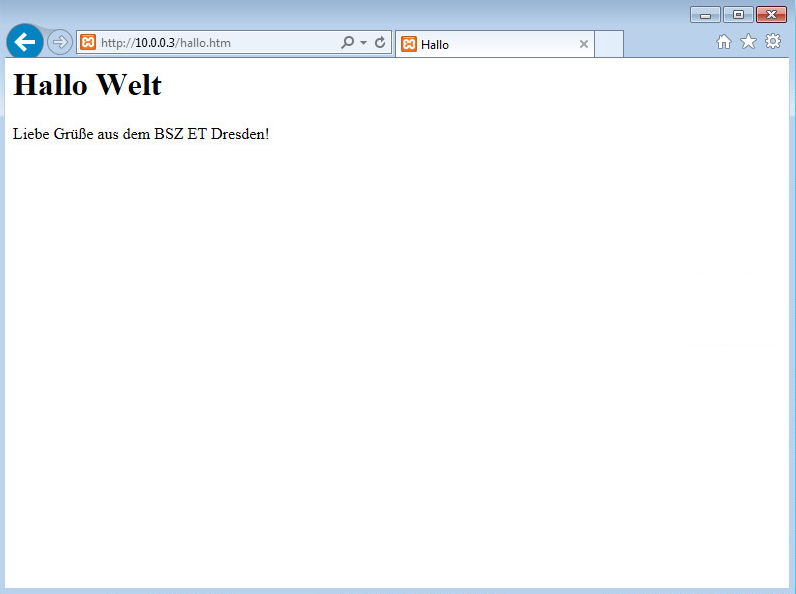
\includegraphics[width=0.7\textwidth]{2_1_1/02.PNG}
        \source{Instellation mit XAMPP Wizard}{Screenshot}{}
    \end{figure}

    \begin{figure}[H]
        \centering
        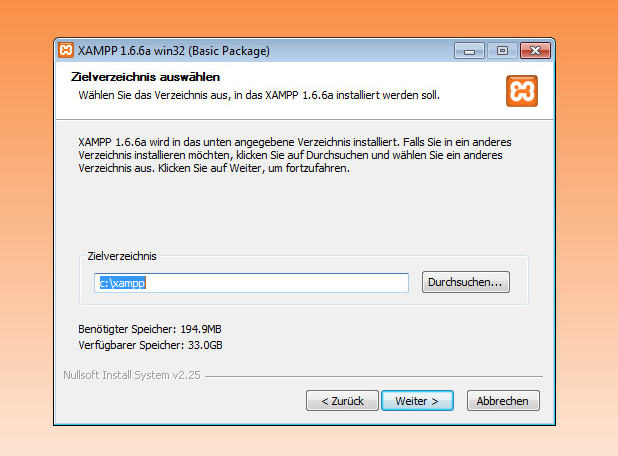
\includegraphics[width=0.7\textwidth]{2_1_1/03.PNG}
        \source{Instellationsverzeichnis}{Screenshot}{}
    \end{figure}

    \begin{figure}[H]
        \centering
        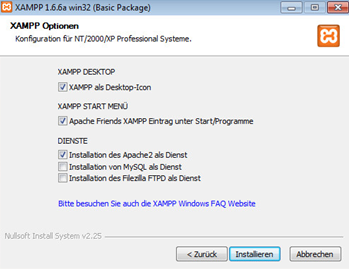
\includegraphics[width=0.7\textwidth]{2_1_1/06_Auswahl.png}
        \source{Konfiguration (Apache)}{Screenshot}{}
    \end{figure}


\subsubsection{Netzwerkfunktionalität beider Workstations}
    \textbf{Planung}
    \begin{itemize}
        \item IPs der WS ermitteln
        \item gegenseitiges pingen der WS
    \end{itemize}

    \begin{figure}[H]
        \centering
        \includegraphics[width=0.7\textwidth]{2_1_2/1.png}
        \source{Ping von Workstation 2 zu Workstation 1}{Screenshot}{}
    \end{figure}

    \begin{figure}[H]
        \centering
        \includegraphics[width=0.7\textwidth]{2_1_2/2.png}
        \source{Ping von Workstation 1 zu Workstation 2}{Screenshot}{}
    \end{figure}


\subsubsection{Netzwerkfunktionalität beider Workstations}
    \textbf{Planung}
    \begin{itemize}
        \item XAMPP installieren 
        \item Apache starten
        \item testen ob Dienst läuft - in browser ip des anderen servers eingeben und prüfen, ob webseite aufgerufen wird 
    \end{itemize}

    \begin{figure}[H]
        \centering
        \includegraphics[width=0.7\textwidth]{2_1_3/1.png}
        \source{hallo.htm nach C:{\textbackslash}xampp{\textbackslash}htdocs kopieren}{Screenshot}{}
    \end{figure}

    \begin{figure}[H]
        \centering
        \includegraphics[width=0.7\textwidth]{2_1_3/2.png}
        \source{Apache in XAMPP Starten}{Screenshot}{}
    \end{figure}

    \begin{figure}[H]
        \centering
        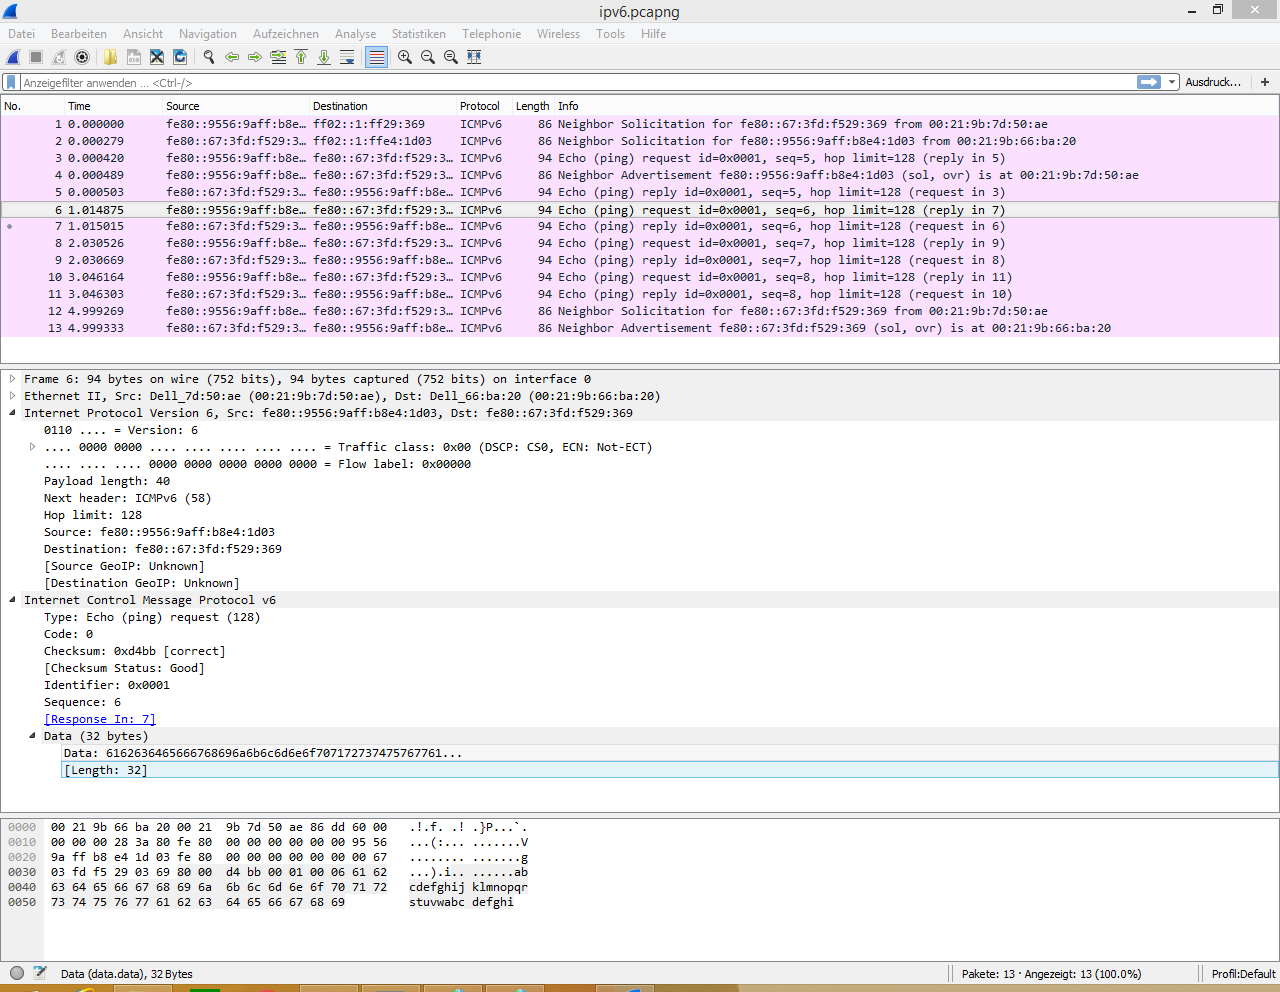
\includegraphics[width=0.7\textwidth]{2_1_3/4.png}
        \source{lokaler Aufruf von hallo.htm}{Screenshot}{}
    \end{figure}

    \begin{figure}[H]
        \centering
        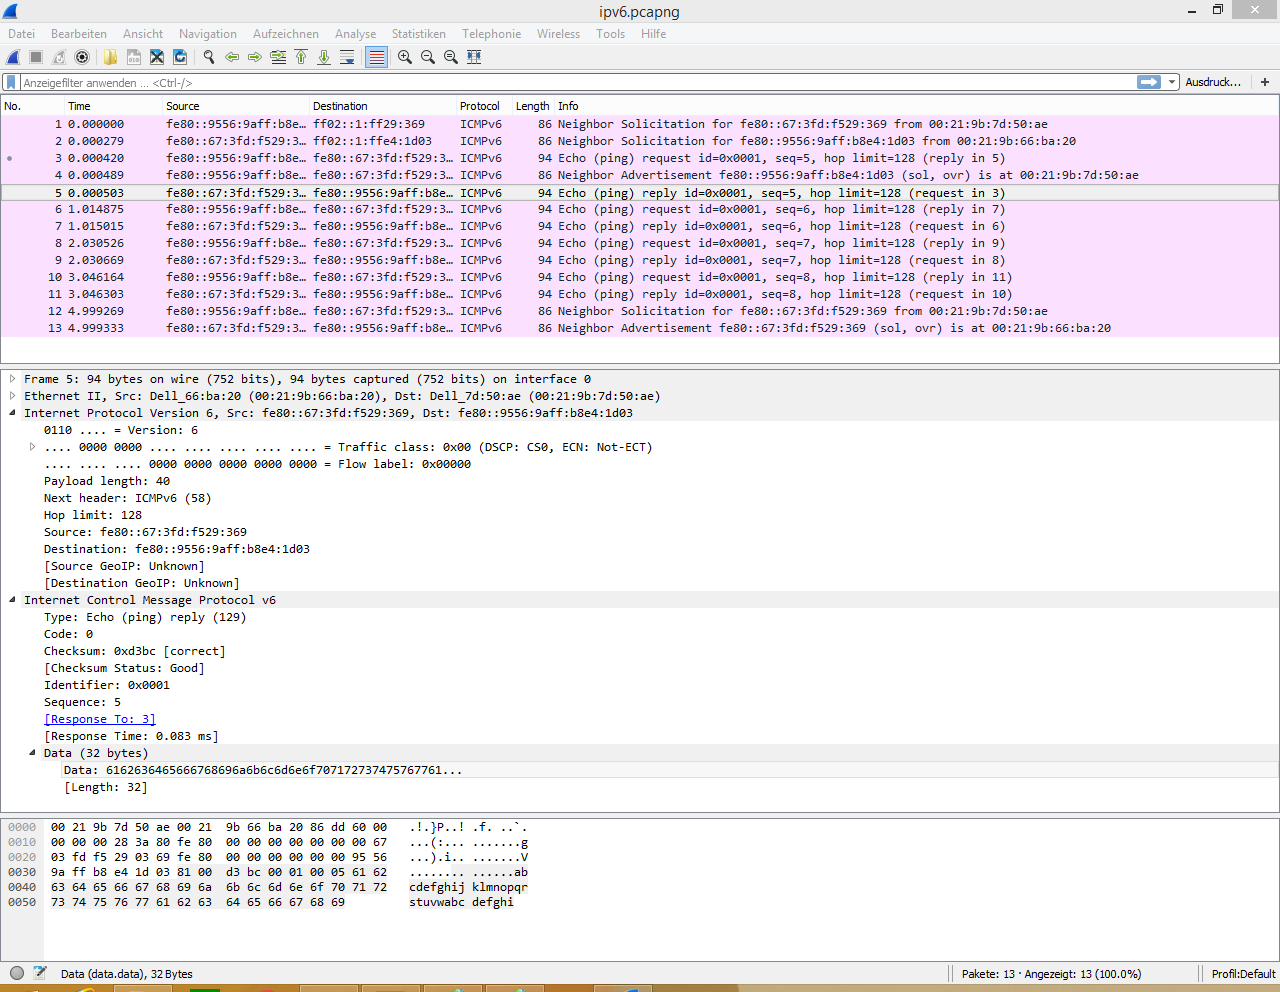
\includegraphics[width=0.7\textwidth]{2_1_3/5.png}
        \source{Aufruf von hallo.htm per IP}{Screenshot}{}
    \end{figure}

\subsubsection{Installieren von Wireshark}
    \begin{figure}[H]
        \centering
        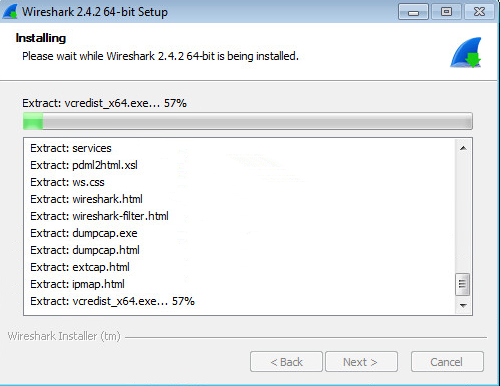
\includegraphics[width=0.7\textwidth]{2_1_4/01.PNG}
        \source{Installation von Wireshark}{Screenshot}{}
    \end{figure}